\section{Survival Analysis}

\subsection{Intro}

\begin{frame}[noframenumbering]{Plan For This Presentation}
  \begin{figure}[h!]
  \centering
    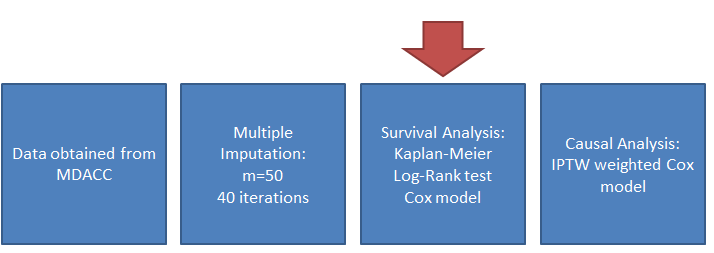
\includegraphics[width=0.9\textwidth]{surv_flow}
\label{fig:surv_flow}
\end{figure} 
\end{frame}

\begin{frame}{Survival Analysis}
\begin{block}{Definition}
Survival analysis is a field of statistics concerned with analyzing time to 
event data, often in the face of censoring or truncation.
\end{block}
Example:
\begin{itemize}
 \item The survival of patients after brain mets from breast cancer
 \item Censoring/Truncation:
 \begin{itemize}
  \item study ending and no death 
  \item subject dies before study starts
  \item subject moves away and can't contact them 
 \item exact death time only known in an interval
 \end{itemize}

\end{itemize}
\end{frame}

\subsection{Kaplan-Meier}
\begin{frame}{Kaplan-Meier Estimator}
\begin{itemize}
 \item The survival function $S(t)=P(T>t)=\int_{t}^{\infty}f(u)du$ is estimated by the 
 nonparametric Kaplan-Meier Estimator
 $$\hat{S}(t)=\prod_{t_i<t}\frac{n_i -d_i}{n_i}$$
\item $n_i$ is the number of subject in the risk set at time $t_i$
\item $d_i$ is the number of deaths at time $t_i$
\end{itemize}
 \begin{figure}[h!]
  \centering
    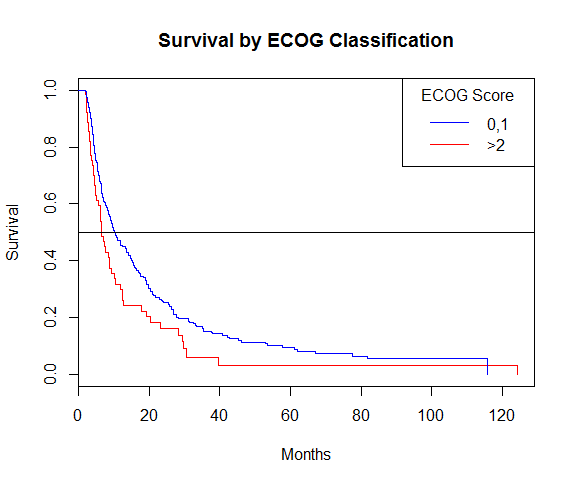
\includegraphics[width=0.33\textwidth]{ecog_km.png}
  \caption{AC Kaplan-Meier Curve for ECOG group}
\label{fig:KMcurve}
\end{figure}
\note{
 risk set at time t; the set of individuals alive and uncensored just before time t.
We use death and survival because easy to say, but it really means event or not}
\end{frame}




\begin{frame}{Kaplan-Meier in the MI Setting}
 \begin{itemize}
  %\item Clearly define the population, groups, and events of interest
  \item Ensure that we have non-informative censoring
\item Algorithm: Pool the complimentary log-log of the Kaplan-Meier curve via Rubin's Rules at
each unique event time, get estimates,
back transform \cite{Marshall2009}
 \end{itemize}
\note{noninformative censoring: knowledge of a censoring time provides no further info about the
persons survival had they not been censored }
\end{frame}

%moved median to extras


\subsection{Log Rank Test}
\begin{frame}{Log Rank test}
$H_0$: No difference between the survival curves of the two populations

$$\frac{\sum_{j=1}^{J}(O_{1j}-E_{1j})}{\sqrt{\sum_{j=1}^{j}V_{j}}}\sim N(0,1)$$
\begin{itemize}
 \item $N_j=N_{1j}+N_{2j}$ is the number at risk at time j (composed from deaths in each group)
 \item $O_j=O_{1j}+O_{2j}$ is the observed number of deaths at time j (composed from the observed deaths in each group)
 \item $E_{1j}=\frac{O_jN_{1j}}{N_j}$
 \item $V_j=\frac{O_j(N_{1j}/N_j)(1-N_{1j}/N_j)(N_{j}-O_{j})}{N_j -1}$
 \end{itemize}
%\note[itemize]{ mention weights?
%}
\end{frame}

\begin{frame}{Log Rank Test in MI Setting}
 \begin{itemize}
 \item Combining tests is usually a bad idea \cite{Marshall2009}
 \item Under no tied times, the score test on
  Cox regression on treatment only is equivalent to the
log rank test
\item Idea: Derive log rank test from Cox regression
%\begin{itemize}
 %\item Pooling LRT and Score test is unstable \cite{Marshall2009}
 %\item Score and Likelihood involve knowing 
%\end{itemize}
 %\item Final Solution: Run the Wald test on Cox regression as an approximation
\item Algorithm: Run Wald test on Cox regression as an approximation to score test
 \end{itemize}
\note{there are lots of issues, I moved them to extras
Might need to check PH assumption on LR test}
\end{frame}

\subsection{KM and Log Rank Application}
\begin{frame}{Chemo KM and Log Rank Test}
  \begin{columns}[onlytextwidth]
    \begin{column}{0.70\textwidth}
	 \begin{figure}[h!]
  \centering
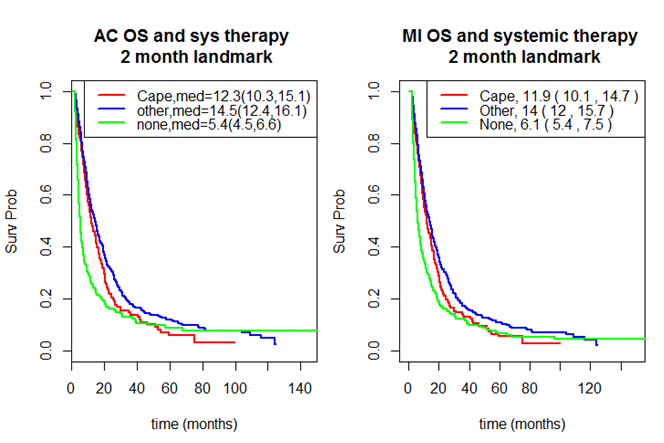
\includegraphics[width=.99\textwidth]{cape_km2}
\end{figure}

    \end{column}
    \begin{column}{0.30\textwidth}
    \begin{table}[]
\centering
\adjustbox{max height=\dimexpr\textheight-5.5cm\relax,
           max width=\textwidth}{
\begin{tabular}{|l|c|c|}
\hline
                & \multicolumn{2}{c|}{Chemo}                         \\ \hline
                & \multicolumn{1}{l|}{AC} & \multicolumn{1}{l|}{MI} \\ \hline
Cape./other/none & \textless.0001          & \textless.0001          \\ \hline
Cape./other      & 0.0321                  & 0.033                   \\ \hline
Cape./none       & 0.00039                 & .0016                   \\ \hline
other/none      & \textless.0001          & \textless.0001          \\ \hline
\end{tabular}
}
\end{table}

    \end{column}

	\end{columns}
\end{frame}



\begin{frame}{HER2 Directed KM and Log Rank Test}
  \begin{columns}[onlytextwidth]
    \begin{column}{0.70\textwidth}
	 \begin{figure}[h!]
  \centering
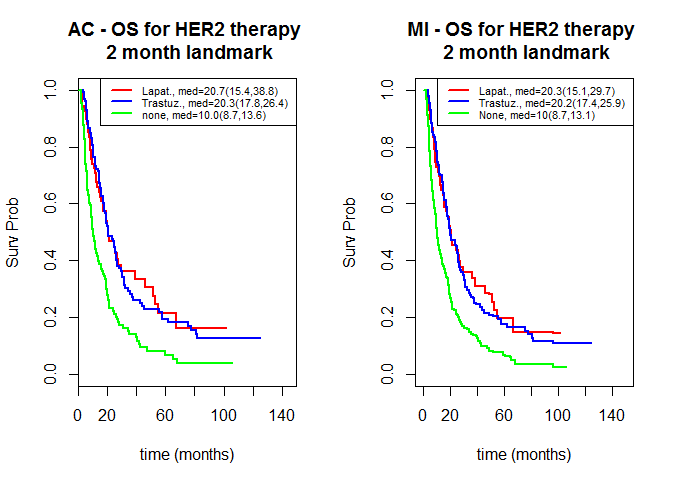
\includegraphics[width=.99\textwidth]{lapat_km}
\end{figure}

    \end{column}
    \begin{column}{0.30\textwidth}
    \begin{table}[]
\centering
\adjustbox{max height=\dimexpr\textheight-5.5cm\relax,
           max width=\textwidth}{
\begin{tabular}{|l|c|c|}
\hline
                   & \multicolumn{2}{c|}{HER2}                         \\ \hline
                   & \multicolumn{1}{l|}{AC} & \multicolumn{1}{l|}{MI} \\ \hline
Lapat./Trastuz./none & \textless.0001          & \textless.0001          \\ \hline
Lapat./Trastuz.      & .87                     & .81                     \\ \hline
Lapat./none         & .00017                  & .00018                  \\ \hline
Trastuz./none       & \textless.0001          & \textless.0001          \\ \hline
\end{tabular}
}
\end{table}

    \end{column}

	\end{columns}
\end{frame}

\subsection{Cox Regression}
\begin{frame}{Cox Regression: Hazard Function}
\begin{itemize}
 \item Hazard is the instantaneous rate of event given that you have survived until time t, given 
 by $$h(t)=\lim_{\Delta t \rightarrow 0+}\frac{P[t\leq T<t+\Delta t|T\geq t]}{\Delta t}$$
\end{itemize}
 \begin{figure}[h!]
  \centering
    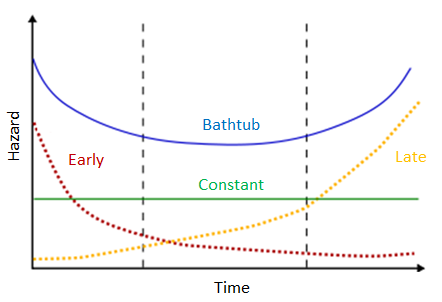
\includegraphics[width=0.55\textwidth]{hazard.png}
  \caption{A few different hazard function shapes \cite{wikihazard}}
\label{fig:hazard}
\end{figure}
\end{frame}

\begin{frame}{Cox Regression}
\begin{itemize}
   \item Cox regression models hazard by 
   
   %$$h(t|Z)=h_{0}(t)\exp(\sum_{k=1}^{p}\beta_{k}Z_{k})$$
   $$h(t|Z)=\underbrace{h_{0}(t)}_{\textrm{time}}*\underbrace{exp(\sum_{k=1}^{p}\beta_{k}Z_{k})}_{\textrm{covariates}}$$

   \item Where $h_{0}(t)$ is the baseline hazard
   \item $Z_k$ is the $k^{th}$ covariate
   \item $\beta_k$'s are found by maximizing the partial likelihood function
\item The covariates act to multiply the hazard function.
\end{itemize}
Quantity of interest: Hazard ratio $\frac{h(t|Z)}{h(t|Z^{*})}=\exp(\sum_{k=1}^{p}\beta_{k}(Z_{k}-Z_{k}^{*}))$
\end{frame}


\begin{frame}{Cox Regression in the MI Setting}
\begin{itemize}
 \item Goal: To get a ``baseline'' Cox regression, then add treatment variables
 \item Need to check for proportional hazards assumption
 \begin{itemize}
  \item Problem:  MI Cox regression doesn't have residuals
  \item Solution: Check assumptions (Schoenfeld residuals) on each MI dataset individually
 \end{itemize}
\item Cox regression is normally distributed, use Rubin's Rules to pool
\item Add treatment covariates, rerun models, pool
\end{itemize}
\end{frame}

\subsection{Cox Regression Application}
\begin{frame}{Schoenfeld Residual Splines}
\begin{figure}[h!]
  \centering
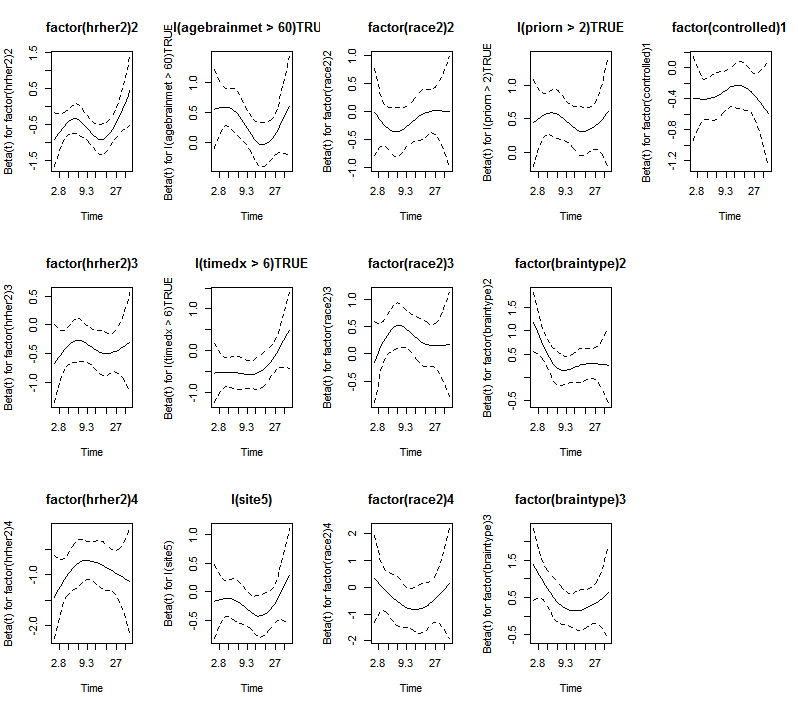
\includegraphics[width=.5\textwidth]{ac_schoenfeld}%
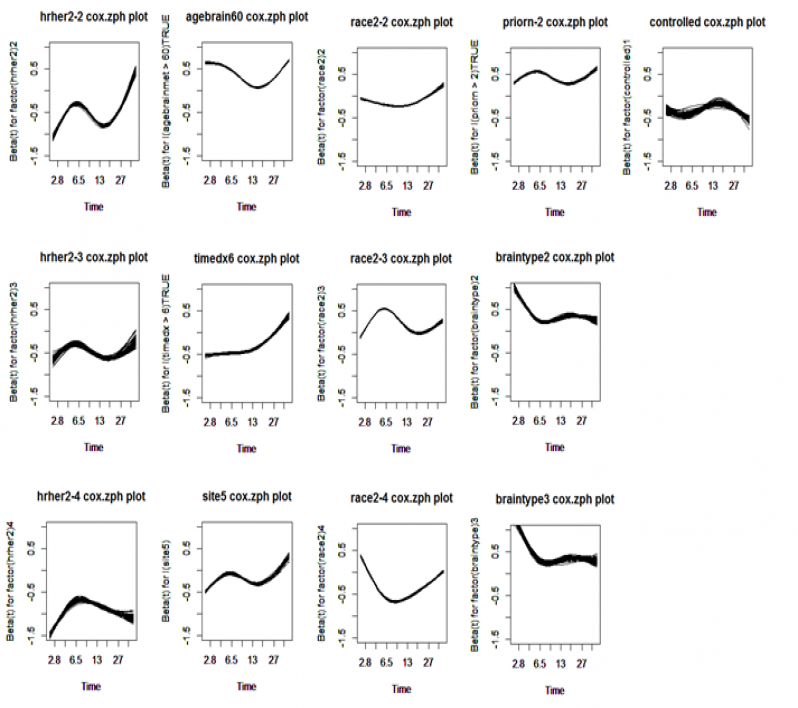
\includegraphics[width=.5\textwidth]{mi_schoenfeld} 
\caption{AC and MI Schoenfeld splines}
\end{figure}
\end{frame}


%moved base model to extras

\begin{frame}{MI Cox Regression, Chemo}
\begin{table}[]
\centering
\adjustbox{max height=.9\dimexpr\textheight-5.5cm\relax,
           max width=\textwidth}{
\begin{tabular}{|l|l|c|c|c|c|c|c|c|}
\hline
                               &                                  &  &  \begin{tabular}[c]{@{}c@{}}AC\\ n= 745\end{tabular}& \multicolumn{1}{l|}{} & \multicolumn{1}{l|}{} & \multicolumn{1}{l|}{} & MI          & \multicolumn{1}{l|}{}                                       \\ \hline
\multicolumn{1}{|c|}{Variable} & \multicolumn{1}{c|}{Contrast}    & HR                                                  & 95\% CI               & p-value               & \multicolumn{1}{l|}{} & HR                    & 95\% CI     & \begin{tabular}[c]{@{}c@{}}p-value \\ (t test)\end{tabular} \\ \hline
HR/HER2                        & -/+ vs. -/-                      & 0.62                                                & (0.49,0.79)           & \textless .0001       &                       & 0.63                  & (0.51,0.77) & \textless .0001                                             \\ \hline
                               & +/- vs. -/-                      & 0.65                                                & (0.53,0.81)           & 0.00011               &                       & 0.64                  & (0.53,0.78) & \textless .0001                                             \\ \hline
                               & +/+ vs. -/-                      & 0.41                                                & (0.31,0.53)           & \textless .0001       &                       & 0.42                  & (0.34,0.53) & \textless .0001                                             \\ \hline
Age                            & \textgreater 60 vs. \textless 60 & 1.34                                                & (1.10,1.64)           & 0.0041                &                       & 1.44                  & (1.21,1.72) & \textless .0001                                             \\ \hline
Dx to BM                       & \textgreater 6 vs. \textless 6   & 0.72                                                & (0.58,0.90)           & 0.0032                &                       & 0.71                  & (0.58,0.86) & 0.00039                                                     \\ \hline
First DM                       & Brain vs. Oth                    & 0.77                                                & (0.63,0.95)           & 0.014                 &                       & 0.81                  & (0.68,0.96) & 0.016                                                       \\ \hline
Race                           & Hisp. Vs. White                  & 0.77                                                & (0.61,0.98)           & 0.034                 &                       & 0.86                  & (0.69,1.06) & 0.15                                                        \\ \hline
                               & Black vs. White                  & 1.29                                                & (1.02,1.63)           & 0.032                 &                       & 1.23                  & (1.01,1.51) & 0.043                                                       \\ \hline
                               & Other vs. White                  & 0.76                                                & (0.47,1.25)           & 0.28                  &                       & 0.7                   & (0.45,1.08) & 0.11                                                        \\ \hline
\# prior Rx                    & \textgreater2 vs. 0-2            & 1.61                                                & (1.32,1.98)           & \textless .0001       &                       & 1.53                  & (1.28,1.82) & \textless .0001                                             \\ \hline
BM type                        & Mult. Vs. Single                 & 1.46                                                & (1.20,1.78)           & 0.00017               &                       & 1.51                  & (1.27,1.81) & \textless .0001                                             \\ \hline
                               & LMD vs. Single                   & 1.45                                                & (1.04,2.03)           & 0.029                 &                       & 1.41                  & (1.11,1.80) & 0.0049                                                      \\ \hline
Sys. Cont.                     & Yes vs. No                       & 0.57                                                & (0.48,0.68)           & \textless .0001       &                       & 0.69                  & (0.59,0.80) & \textless .0001                                             \\ \hline
\rowcolor[HTML]{FE0000} 
Chemo                          & Cape. vs. none                   & 0.69                                                & (0.53,0.89)           & 0.0046                &                       & 0.75                  & (0.60,0.95) & 0.018                                                       \\ \hline
\rowcolor[HTML]{FE0000} 
                        
                        & other vs. none                   & 0.52                                                & (0.42,0.65)           & \textless .0001       &                       & 0.58                  & (0.47,0.71) & \textless .0001                                             \\ \hline
\end{tabular}
}
\caption{AC and MI Cox regression with Chemo Treatment}
\label{acmi_cox_chemo}
\end{table} 
\note{p vals are 0.018 and <.0001}
\end{frame}


\begin{frame}{MI Cox Regression, HER2-Directed}
\begin{table}[]
\centering
\adjustbox{max height=\dimexpr\textheight-5.5cm\relax,
           max width=\textwidth}{
\begin{tabular}{|l|l|c|c|c|c|c|c|c|}
\hline
                               &                                  & \multicolumn{1}{l|}{} & \begin{tabular}[c]{@{}c@{}}AC\\ n=292\end{tabular} & \multicolumn{1}{l|}{} & \multicolumn{1}{l|}{} &      & \begin{tabular}[c]{@{}c@{}}MI\\ n between 391\\ and 415\end{tabular} & \multicolumn{1}{l|}{}                                       \\ \hline
\multicolumn{1}{|c|}{Variable} & \multicolumn{1}{c|}{Contrast}    & HR                    & 95\% CI                                            & p-value               &                       & HR   & 95\% CI                                                              & \begin{tabular}[c]{@{}c@{}}p-value \\ (t test)\end{tabular} \\ \hline
HR/HER2                        & +/+ vs. -/+                      & 0.65                  & (0.49,0.87)                                        & 0.0036                &                       & 0.66 & (0.51,0.85)                                                          & 0.0015                                                      \\ \hline
Age                            & \textgreater 60 vs. \textless 60 & 1.38                  & (0.95,2.01)                                        & 0.092                 &                       & 1.58 & (1.15,2.18)                                                          & 0.0054                                                      \\ \hline
Dx to BM                       & \textgreater 6 vs. \textless 6   & 0.64                  & (0.43,0.97)                                        & 0.033                 &                       & 0.69 & (0.49,0.99)                                                          & 0.041                                                       \\ \hline
First DM                       & Brain vs. Oth                    & 0.84                  & (0.58,1.20)                                        & 0.34                  &                       & 0.86 & (0.62,1.17)                                                          & 0.34                                                        \\ \hline
Race                           & Hisp. Vs. White                  & 0.69                  & (0.46,1.02)                                        & 0.064                 &                       & 0.76 & (0.53,1.09)                                                          & 0.14                                                        \\ \hline
                               & Black vs. White                  & 1.41                  & (0.94,2.11)                                        & 0.1                   &                       & 1.43 & (1.00,2.04)                                                          & 0.047                                                       \\ \hline
                               & Other vs. White                  & 0.7                   & (0.32,1.53)                                        & 0.38                  &                       & 0.83 & (0.46,1.52)                                                          & 0.55                                                        \\ \hline
\# prior Rx                    & \textgreater2 vs. 0-2            & 1.88                  & (1.34,2.63)                                        & 0.00028               &                       & 1.71 & (1.28,2.28)                                                          & 0.00028                                                     \\ \hline
BM type                        & Mult. Vs. Single                 & 1.3                   & (0.92,1.86)                                        & 0.14                  &                       & 1.25 & (0.91,1.70)                                                          & 0.16                                                        \\ \hline
                               & LMD vs. Single                   & 2.15                  & (1.20,3.88)                                        & 0.011                 &                       & 1.77 & (1.10,2.83)                                                          & 0.018                                                       \\ \hline
Sys. Cont.                     & Yes vs. No                       & 0.73                  & (0.55,0.97)                                        & 0.029                 &                       & 0.78 & (0.60,1.01)                                                          & 0.063                                                       \\ \hline
\rowcolor[HTML]{FE0000} 
HER2 therapy                   & Lapat. vs. none                   & 0.47                  & (0.32,0.69)                                        & 0.00015               &                       & 0.52 & (0.37,0.75)                                                          & 0.00036                                                     \\ \hline
\rowcolor[HTML]{FE0000} 

                               & Trastuz. vs. none                 & 0.45                  & (0.33,0.61)                                        & \textless.0001        &                       & 0.51 & (0.38,0.68)                                                          & \textless.0001                                              \\ \hline
\end{tabular}
}
\caption{AC and MI Cox regression with HER2 Treatment}

\end{table}
\note{p vals are 0.00036 and <.0001}
\end{frame}